\subsection{Laufrichtungen kombinieren}
Die Charaktersteuerung benötigt je nach Tastatureingabe eine unterschiedliche Bewegungsrichtung. Der Unity ML-Agents Agent enthält eine Funktion zum wechseln des verwendeten Modells. Mit dieser Funktion wird in folgender Implementierung zwischen den seperaten Bewegungsmodellen gewechselt um alle Bewegungsrichtungen mit einer Steuerung abzudecken. Zu Erwarten ist das die Bewegung in die einzelnen Richtungen funktioniert, der Läufer aber beim Wechsel zwischen den Modellen das Gleichgewicht nicht halten kann.

\begin{lstlisting}[caption={Laufrichtung Modell wechseln},captionpos=b,label={lst:laufrichtung_modell_wechsel}]
public override void FixedUpdate() {
    ...    
    agent.targetWalkingSpeed = 5f;
    if (inputVert != 0) //Tastatur Input Vor oder Zurück
    {
        // Vorwärts
        if (inputVert > 0)
        {
            agent.SetModel("Walker", modelForward);
        }
        else // Zurück
        {
            agent.SetModel("Walker", modelBackward);
        }
    }
    else if (inputHor != 0) // Links oder Rechts
    {
        if (inputHor > 0) // Rechts
        {
            agent.SetModel("Walker", modelRight);
        }
        else // Links
        {
            agent.SetModel("Walker", modelLeft);
        }
    }
    else //kein Input -> Auf der Stelle stehen
    {
        agent.targetWalkingSpeed = 0f;
        agent.SetModel("Walker", modelStanding);
    }
    ...
}
\end{lstlisting}

Wie angenommen funktioniert das Bewegen in eine konstante Richtung gut. Beim Wechsel zu einem anderen Modell fällt der Läufer ohne Ausnahme.

Der erste Versuch alle Bewegungsrichtungen in einem Modell anzulernen, wurde von den Methoden der Walker Demo inspiriert. Gleich wie das Laufziel wurde ein zusätzliches Zielobjekt hinzugefügt, welches zufällig platziert wurde. Um die Komplexität nicht von Anfang an zu hoch anzusetzen, wurde das Blickziel zu beginn die Winkelabweichung zwischen Zielrichtung und Blickrichtung langsam über ein Lehrplan angepasst. Anfangs wurde das Blickziel mit einer Winkelabweichung im Bereich von -5 und 5 Grad platziert, zum Ende hin wurde der Bereich immer weiter bis auf -90 bis 90 Grad erweitert (siehe Codeausschnitt \ref{lst:lehrplan_blickziel}). Das Blickziel wurde neu gesetzt sobald ein Ziel erreicht wurde.

\begin{lstlisting}[caption={ Lehrplan für das Blickziel},captionpos=b,label={lst:lehrplan_blickziel}]
lookAngleLimit:
    curriculum:
      - name: min max 5 degree look target deviation
        completion_criteria:
          measure: progress
          behavior: Walker
          threshold: 0.4
          signal_smoothing: true
        value: 5.0
      - name: min max 30 degree look target deviation
        completion_criteria:
          measure: progress
          behavior: Walker
          threshold: 0.6
          signal_smoothing: true
          require_reset: true
        value: 30.0
      - name: min max 60 degree look target deviation
        completion_criteria:
          measure: progress
          behavior: Walker
          threshold: 0.8
          signal_smoothing: true
          require_reset: true
        value: 60.0
      - name: min max 90 degree look target deviation
        completion_criteria:
          measure: progress
          behavior: Walker
          threshold: 1.0
          signal_smoothing: true
          require_reset: true
        value: 90.0
\end{lstlisting}

Der Läufer lernt einen stabilen Gang (siehe Abbildungen \ref{fig:103_move_target_dir} und \ref{fig:103_reach_target}). Die Winkelabweichung von 5 Grad ist mit aktueller Belohnungsfunktion jedoch nahezu zu vernachlässigen. Vor folgenden Lehreinheiten hat sich bereits ein Verhalten so start gefestigt, das die Lehreinheiten keine Wirkung zeigen (siehe Abbildungen \ref{fig:103_look_angle_limit} und \ref{fig:126_look_reward}.

\begin{figure}[H]
  \centering  
    \begin{subfigure}{.49\textwidth}
      \centering  
      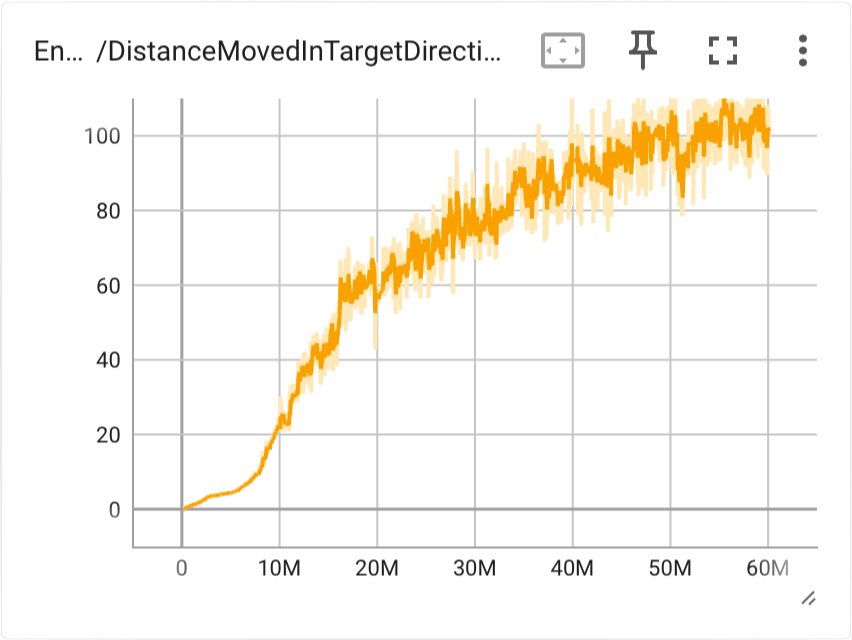
\includegraphics[width=\textwidth]{img/103_move_target_dir}
      \caption{Zurückgelegte Strecke in Zielrichtung}
      \label{fig:103_move_target_dir}
    \end{subfigure}
    \begin{subfigure}{.49\textwidth}
      \centering  
      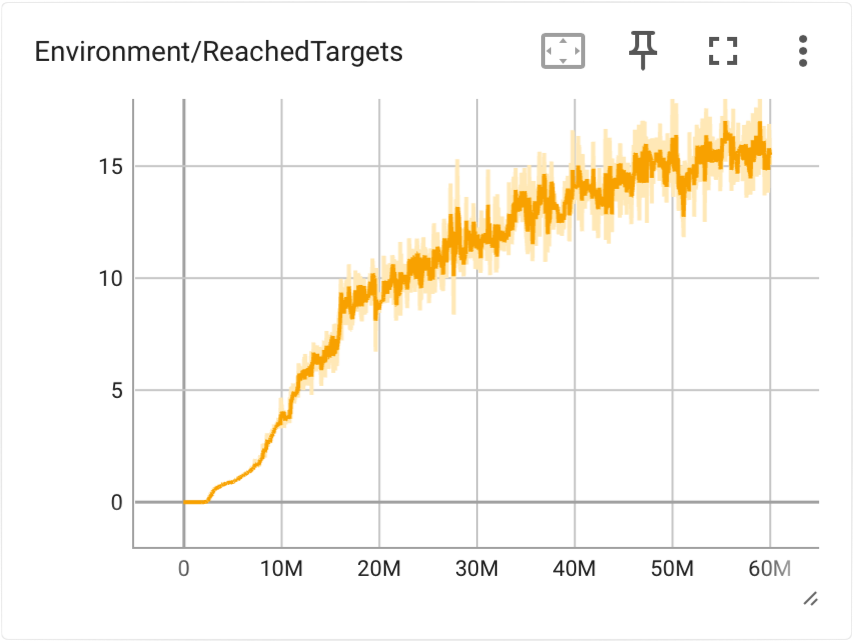
\includegraphics[width=\textwidth]{img/103_reach_target}
      \caption{Erreichte Anzahl an Zielen}
      \label{fig:103_reach_target}
    \end{subfigure}
    \begin{subfigure}{.49\textwidth}
      \centering  
      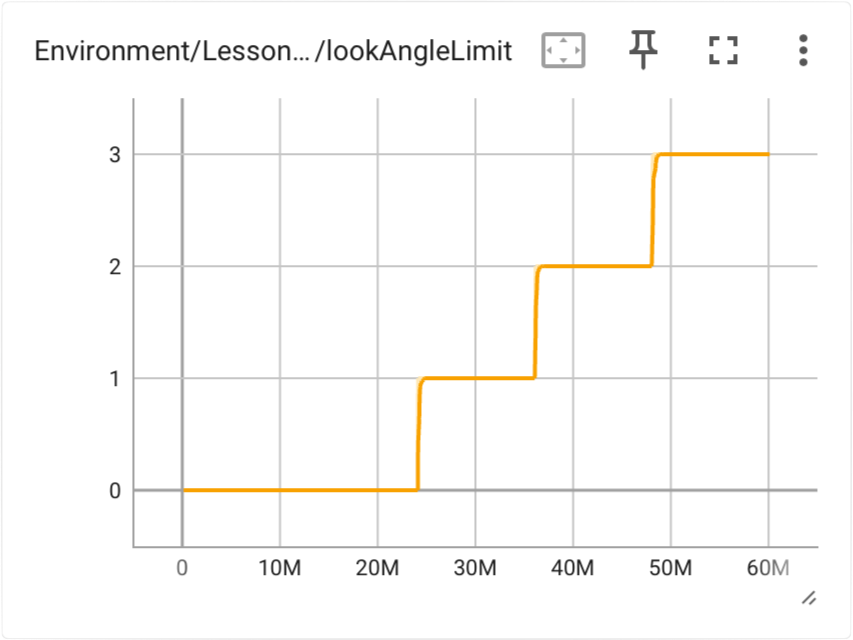
\includegraphics[width=\textwidth]{img/103_look_angle_limit}
      \caption{Aktive Lehreinheit}
      \label{fig:103_look_angle_limit}
    \end{subfigure}
     \begin{subfigure}{.49\textwidth}
      \centering  
      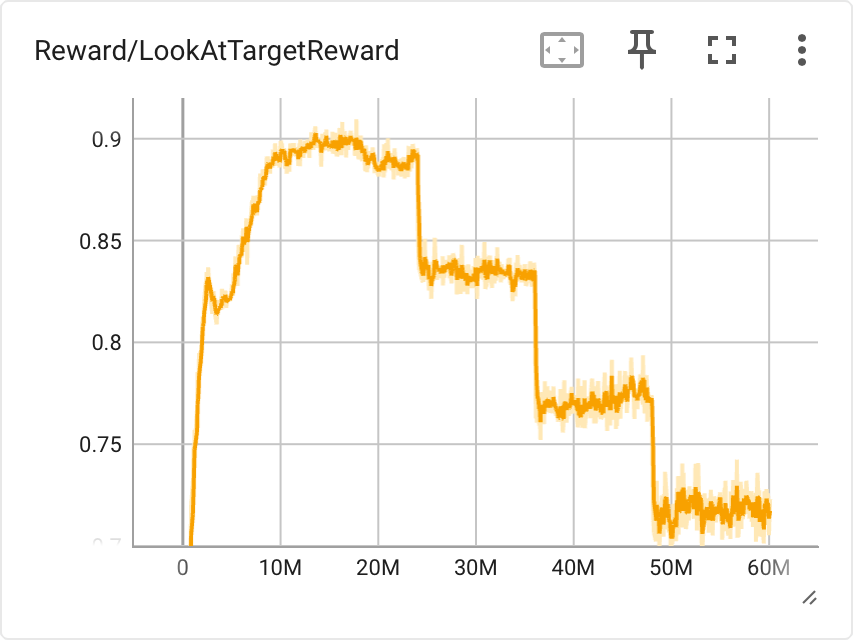
\includegraphics[width=\textwidth]{img/103_look_reward}
      \caption{Blickbelohnung}
      \label{fig:103_look_reward}
    \end{subfigure}
  \caption{Training Blickrichtungsziel mit Lehrplan}
  \label{fig:training_blickrichtungsziel_lehrplan}
\end{figure}

Um von Beginn an ein generell gültiges Verhalten anzutrainieren, wurden Trainings ohne Lehrplan durchgeführt. Dabei wurde ein Training mit einer Winkelabweichung von +-90 Grad und eins mit +-180 Grad durchgeführt. Der Läufer lernt bei beiden Trainings kaum die Blickrichtung der neuen Zielblickrichtung anzupassen. Bei Training mit Winkelabweichungen von bis zu +-180 Grad lernt der Läufer negative Belohnungen mit einer Blickrichtung vertikal nach unten zu umgehen. Dies ist möglich da die die Blickrichtung Vertikal nach unten entlang der Y-Achse verläuft. Bei der Berechnung der Blickbelohnung wird die Y-Komponente der Blickrichtung auf 0 gesetzt, da die Zielrichtung auch ohne Höhenkomponente festgelegt wird um Höhenunterschiede zwischen Hüfte und Ziel zu ignorieren. Durch dieses Schlupfloch kann der Läufer negative Belohnungen verhindern ohne die Gangart nennenswert anzupassen.

\begin{figure}[H]
  \centering  
    \begin{subfigure}{.49\textwidth}
      \centering  
      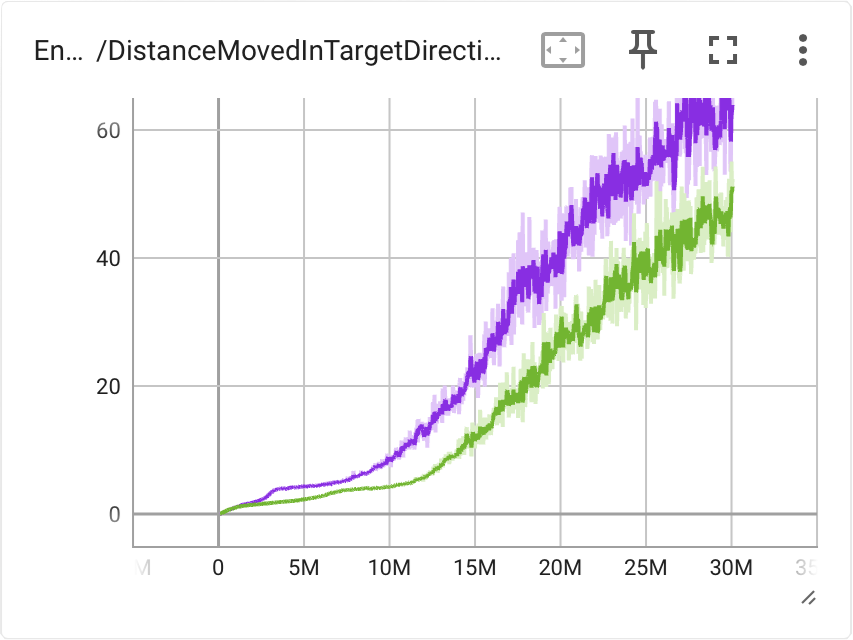
\includegraphics[width=\textwidth]{img/104_105_move_target_dir}
      \caption{Zurückgelegte Strecke in Zielrichtung}
      \label{fig:104_105_move_target_dir}
    \end{subfigure}
    \begin{subfigure}{.49\textwidth}
      \centering  
      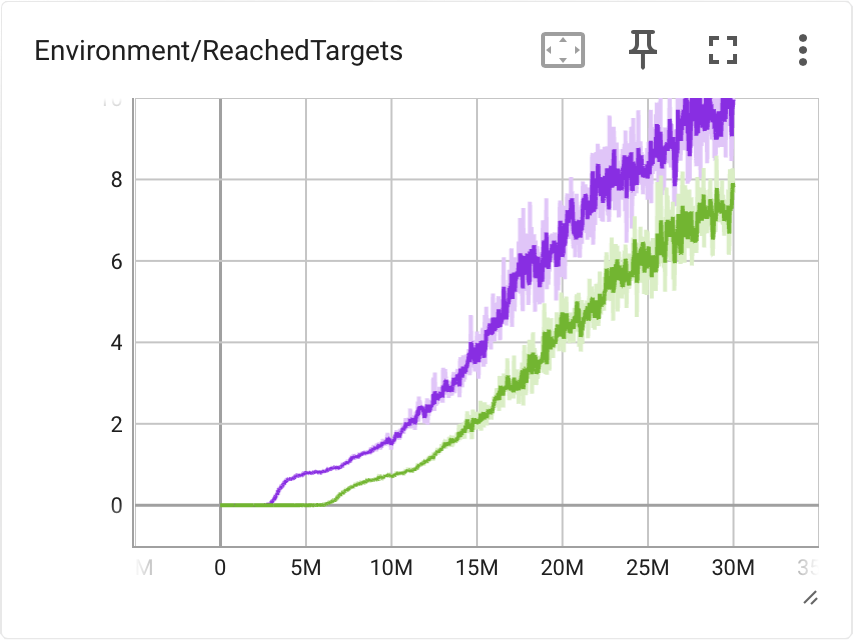
\includegraphics[width=\textwidth]{img/104_105_reach_target}
      \caption{Erreichte Anzahl an Zielen}
      \label{fig:104_105_reach_target}
    \end{subfigure}
    \begin{subfigure}{.49\textwidth}
      \centering  
      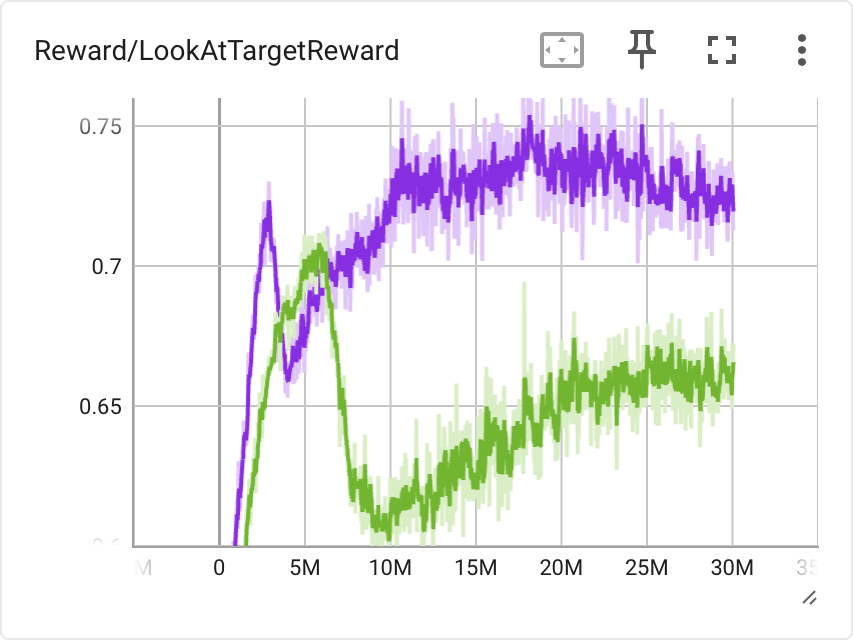
\includegraphics[width=\textwidth]{img/104_105_look_reward}
      \caption{Blickbelohnung}
      \label{fig:104_105_look_reward}
    \end{subfigure}
  \caption{Training Blickrichtungsziel (blau = Winkelabweichung +-90 Grad, grün = Winkelabweichung +-180 Grad)}
  \label{fig:training_blickrichtungsziel}
\end{figure}

Um das Schlupfloch der Blickbelohnung zu stopfen wird eine neue Bestrafung eingeführt. Die Kopfneigungsbestrafung bestraft den Läufer für das neigen des Kopfs und sorgt somit dafür das der Läufer den Kopf aufrecht hält. Im Training mit der neuen Kopfneigungsbestrafung lernt der Läufer langsamer und findet eine neuen Ausweg die Belohnungen generell gültig zu optimieren ohne unterschiedliche Gangarten zu erlernen. Durch die Eigenschaft des Trainings, dass der Winkel zwischen Läufer, Ziel und Blickziel nur bei der Platzierung des Blickziels eingehalten werden, werden die Winkel durch das annähern des Läufers zum Ziel ausnahmslos größer. Somit ist die beste Lösung für den Läufer sich rückwärts zu bewegen, denn so ist die Wahrscheinlichkeit das die Winkelabweichung kleiner ist wesentlich höher (siehe Abbildung \ref{fig:blickwinkel_änderung}).

\begin{figure}[H]
  \centering  
    \begin{subfigure}{.3\textwidth}
      \centering  
      \includegraphics[width=\textwidth]{img/blickwinkel_änderung1}
    \end{subfigure}
    \begin{subfigure}{.3\textwidth}
      \centering  
      \includegraphics[width=\textwidth]{img/blickwinkel_änderung2}
    \end{subfigure}
    \begin{subfigure}{.3\textwidth}
      \centering  
      \includegraphics[width=\textwidth]{img/blickwinkel_änderung3}
    \end{subfigure}
  \caption{Blickwinkel Änderung durch Zielannäherung}
  \label{fig:blickwinkel_änderung}
\end{figure}

Das Problem wurde behoben, indem das Blickziel in nachfolgenden Trainings kontinuierlich mit jedem Update neu platziert wurde, um somit den Blickwinkel gleich zu halten. In den bisherigen Trainingseinheiten hat der Läufer zudem eine Gangart optimiert um allen Blickziele mittelmäßig zu erreichen. Um den Läufer zu motivieren alle Blickziele stärker einzuhalten, wurde die Implementierung geändert, sodass der Blickwinkel beim erreichen des Laufziels nur noch gewechselt wird wenn die Durchschnittliche Blickbelohnung über dem Schwellenwert von 0.7 liegt. Mit dieser neuen Bedingung beim erreichen des Blickziels, erreicht der Läufer die ersten Blickziele und stagniert dann an den neuen Blickzielen (siehe \ref{fig:training_blickrichtungsziel_wechsel_07}).

\begin{figure}[H]
  \centering  
    \begin{subfigure}{.49\textwidth}
      \centering  
      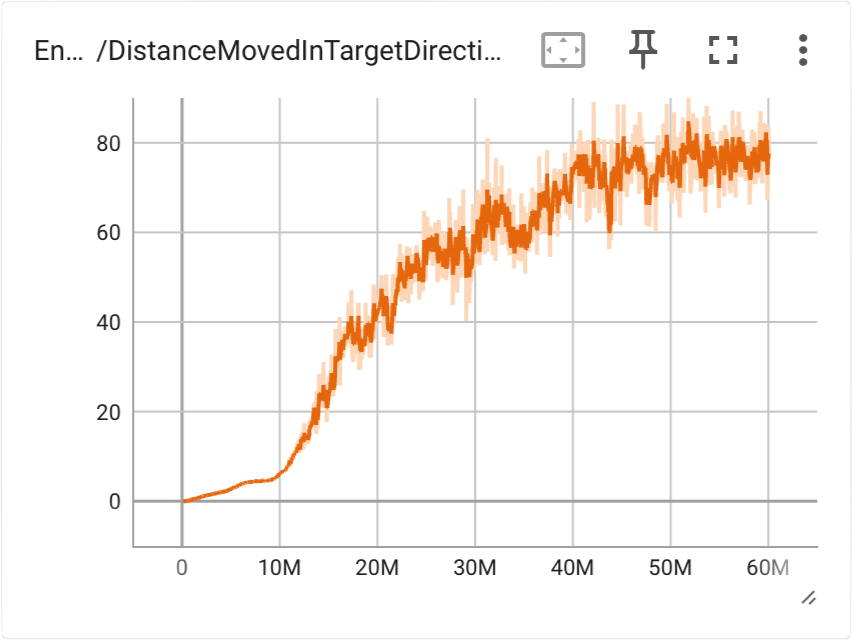
\includegraphics[width=\textwidth]{img/113_move_target_dir}
      \caption{Zurückgelegte Strecke in Zielrichtung}
      \label{fig:113_move_target_dir}
    \end{subfigure}
    \begin{subfigure}{.49\textwidth}
      \centering  
      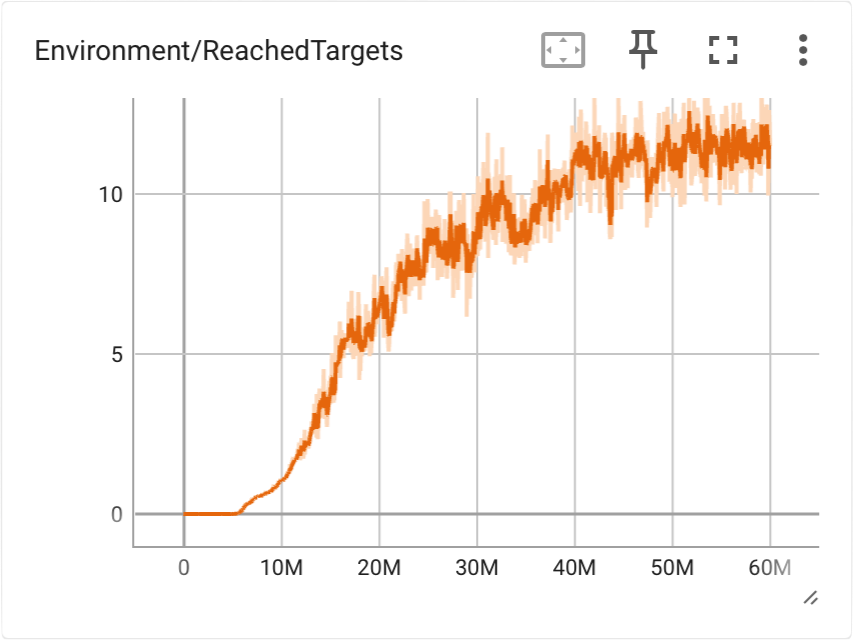
\includegraphics[width=\textwidth]{img/113_reach_target}
      \caption{Erreichte Anzahl an Zielen}
      \label{fig:113_reach_target}
    \end{subfigure}
    \begin{subfigure}{.49\textwidth}
      \centering  
      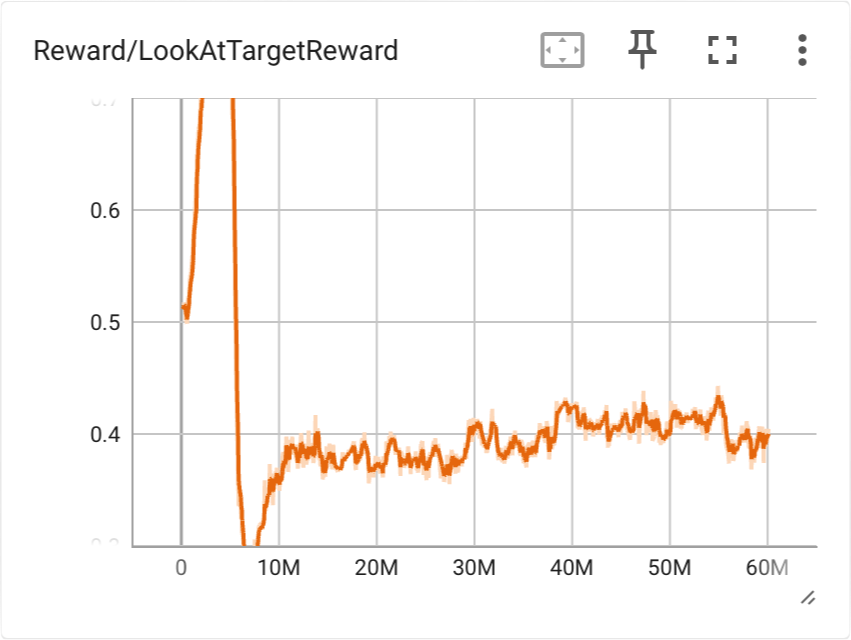
\includegraphics[width=\textwidth]{img/113_look_reward}
      \caption{Blickbelohnung}
      \label{fig:113_look_reward}
    \end{subfigure}
  \caption{Training Blickrichtungsziel mit Wechsel bei durchschnittlicher Blickbelohnung von 0.7}
  \label{fig:training_blickrichtungsziel_wechsel_07}
\end{figure}

Der Läufer braucht zu beginn eine ganze Weile um zu lernen sich bis zum Ziel zu bewegen. Aus diesem Grund verbringt der Läufer auch mit der neuen Bedingung zum erreichen des Blickziels zu viel Zeil des Trainings mit gleichbleibenden Blickzielwinkeln. Um von Anfang an und separat vom erlernen des Laufens die Blickbelohnung zu erlernen, wird die Bedingung für das Erreichen eines Blickziels erneut angepasst. Im folgenden Versuch wird der Blickzielwinkel gewechselt sobald der Läufer 3 Sekunden auf das Ziel blickt. Implementiert wurde das ganze mit einem Spherecast um gleichzeitig zu ermöglichen die Genauigkeit mit der der Läufer auf das Ziel schauen muss anpassen zu können (siehe Abbildung \ref{fig:spherecast}).

\begin{figure}[H]
  \centering  
  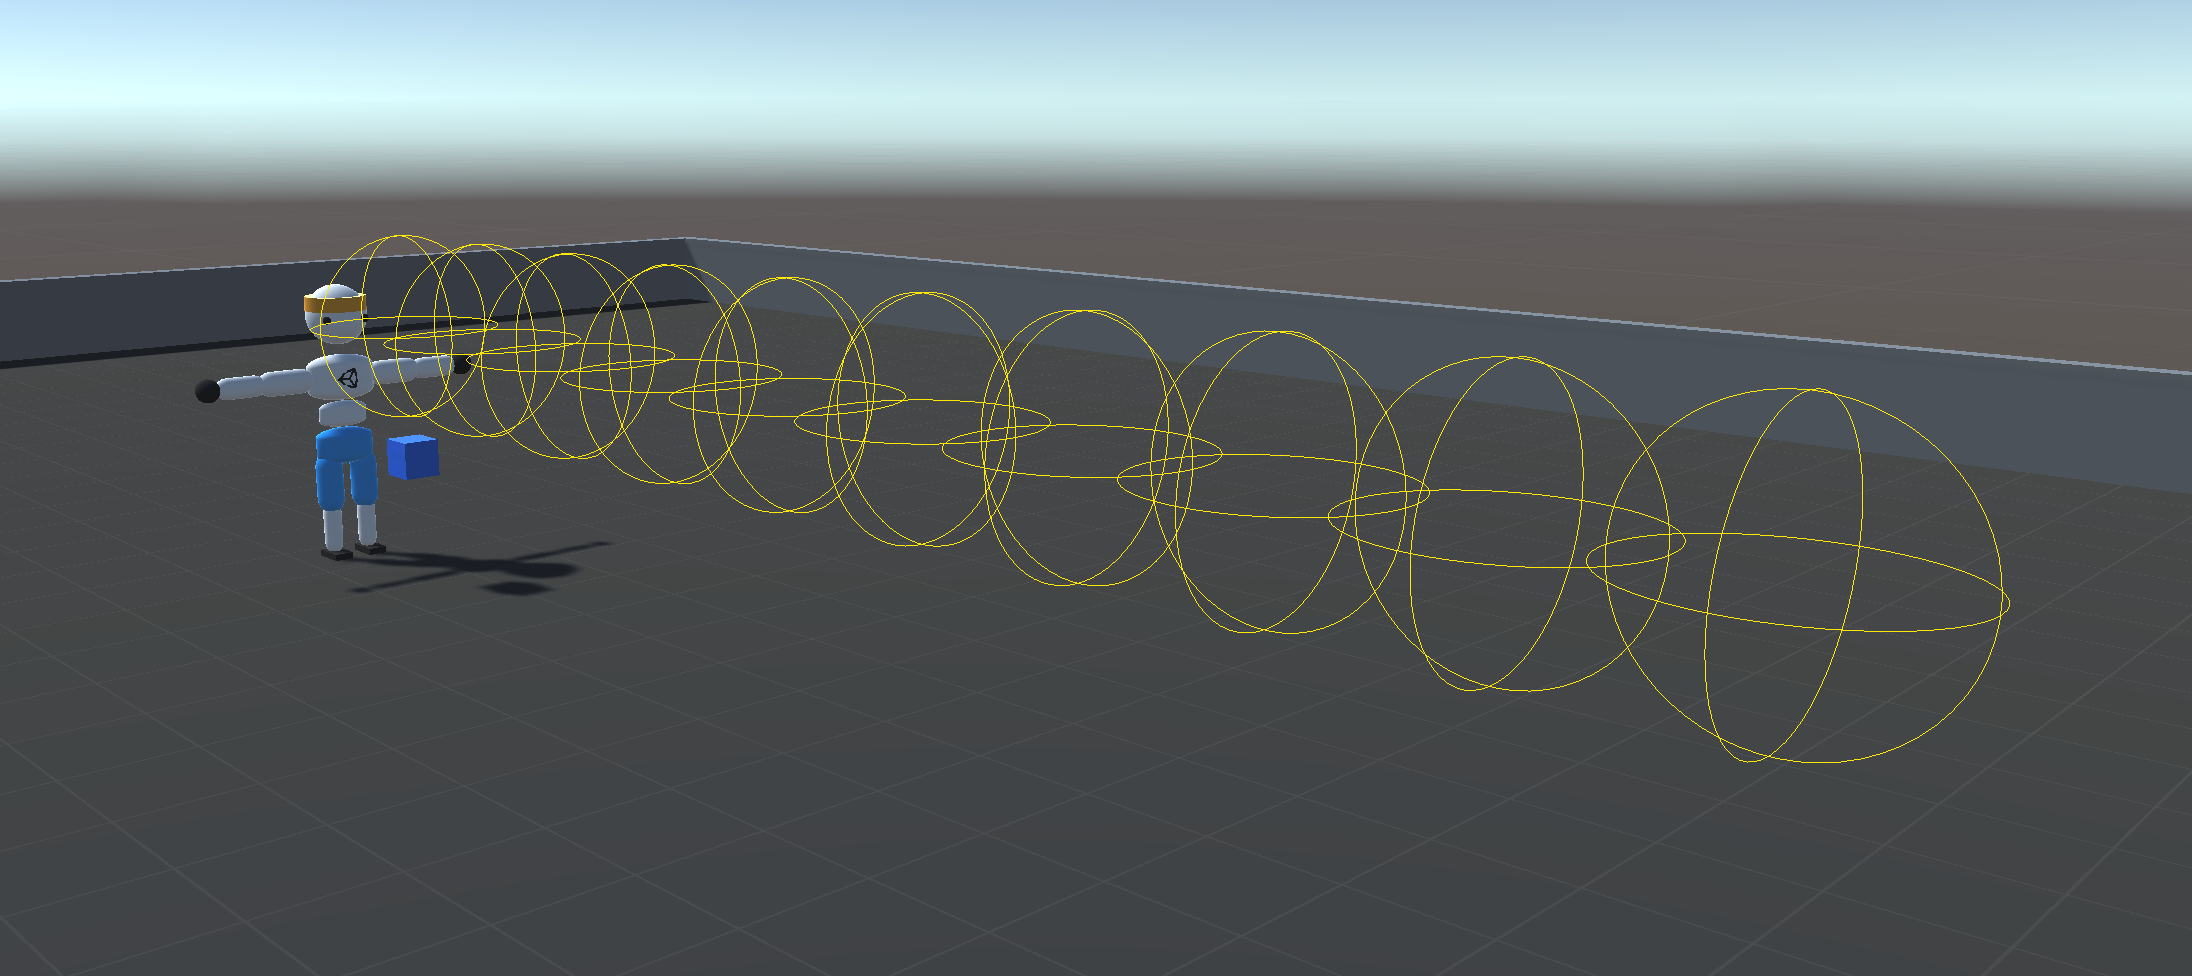
\includegraphics[width=0.8\textwidth]{img/spherecast}
  \caption{Spherecast in Blickrichtung}
  \label{fig:spherecast}
\end{figure}

Das Training wurde einmal mit 3 Sekunden und einmal mit 2 Sekunden Blickkontaktzeit zum erreichen des Blickziels durchgeführt. Wobei das Training mit 2 Sekunden Blickkontaktzeit besser abschneidet. Aber auch das bessere der beiden Trainings ist nach 60 bzw. 120 milionen Trainingsschritten noch weit davon entfernt stabil mehrere Ziele am Stück zu erreichen.

\begin{figure}[H]
  \centering  
    \begin{subfigure}{.49\textwidth}
      \centering  
      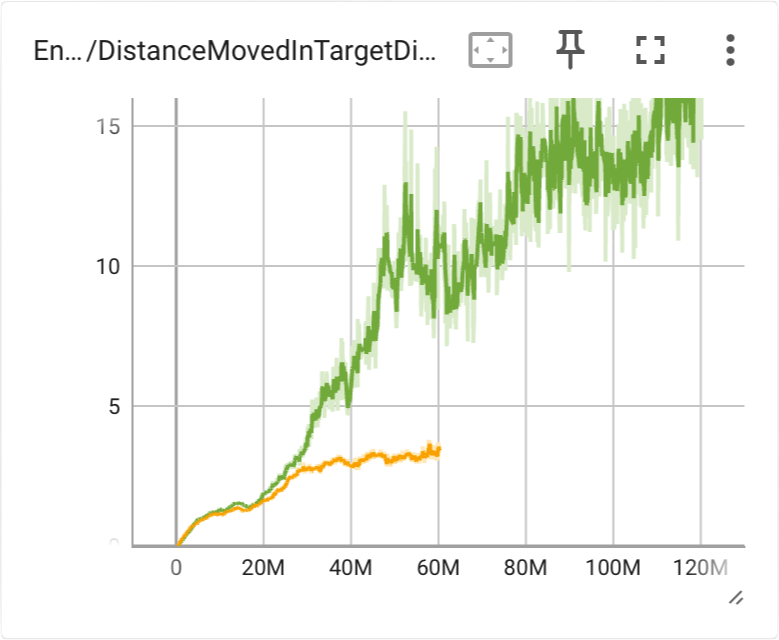
\includegraphics[width=\textwidth]{img/117_119_move_target_dir}
      \caption{Zurückgelegte Strecke in Zielrichtung}
      \label{fig:117_119_move_target_dir}
    \end{subfigure}
    \begin{subfigure}{.49\textwidth}
      \centering  
      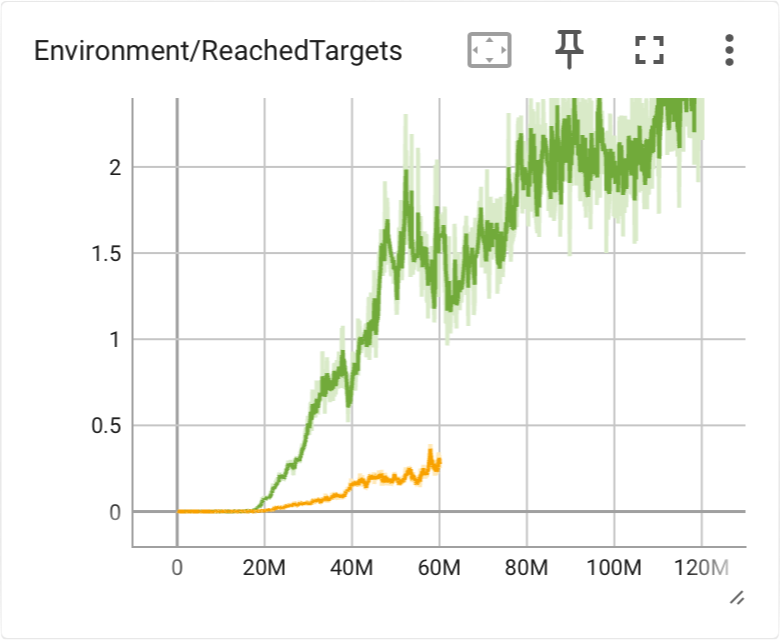
\includegraphics[width=\textwidth]{img/117_119_reach_target}
      \caption{Erreichte Anzahl an Zielen}
      \label{fig:117_119_reach_target}
    \end{subfigure}
    \begin{subfigure}{.49\textwidth}
      \centering  
      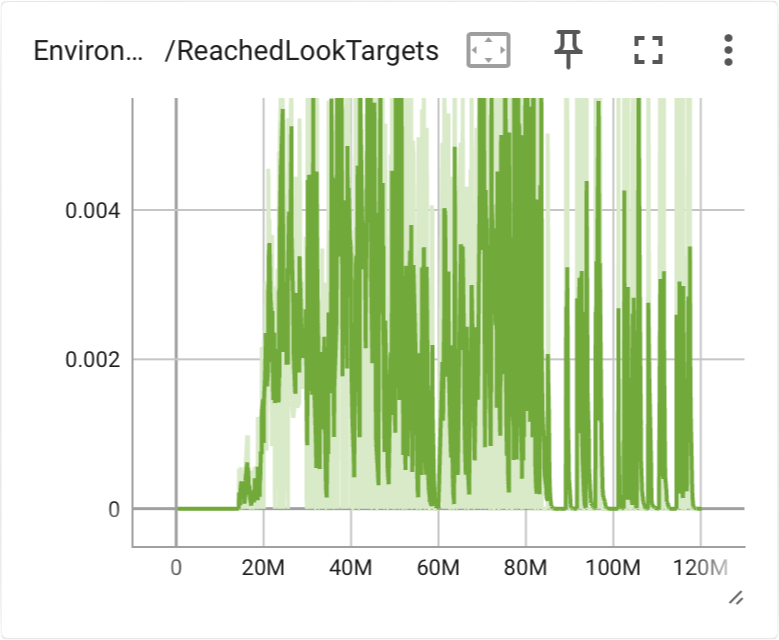
\includegraphics[width=\textwidth]{img/117_119_reach_look_target}
      \caption{Erreichte Anzahl an Blickzielen}
      \label{fig:117_119_reach_look_target}
    \end{subfigure}
    \begin{subfigure}{.49\textwidth}
      \centering  
      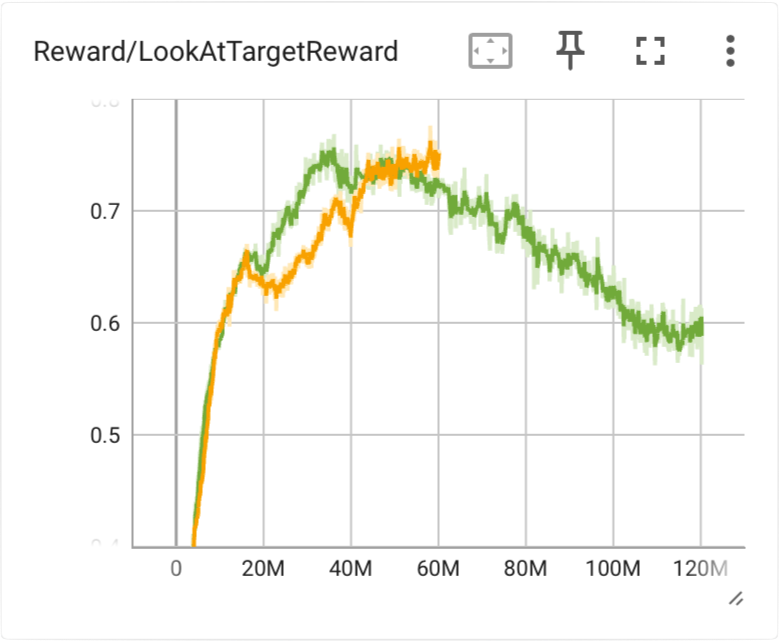
\includegraphics[width=\textwidth]{img/117_119_look_reward}
      \caption{Blickbelohnung}
      \label{fig:117_119_look_reward}
    \end{subfigure}
  \caption{Training Blickrichtungsziel mit Wechsel bei Blickkontakt von 2 bzw. 3 Sekunden (orange = 3 sek, grün = 2 sek)}
  \label{fig:training_blickrichtungsziel_wechsel_spherecast}
\end{figure}